\documentclass[11pt]{article}
\usepackage[utf8]{inputenc}
\usepackage[T1]{fontenc}
\usepackage[margin=1in]{geometry}
\usepackage{amsmath,amssymb}
\usepackage{textcomp}
\usepackage[table]{xcolor}
\definecolor{roblow}{HTML}{C8E6C9}
\definecolor{robsome}{HTML}{FFF1C2}
\definecolor{robhigh}{HTML}{FFCDD2}
\usepackage{graphicx}
\usepackage{booktabs}
\usepackage{longtable}
\usepackage{array}
\usepackage{caption}
\usepackage{float}
\usepackage[hidelinks]{hyperref}
\usepackage{tikz}
\usetikzlibrary{shapes.geometric,arrows.meta,positioning,calc}
\setlength{\parskip}{0.5em}
\setlength{\parindent}{0pt}
\usepackage[numbers,sort&compress]{natbib}
\begin{filecontents*}[overwrite]{\jobname.bib}
@article{Author2013,
  title = {Anodal tDCS improves n-back accuracy over left DLPFC},
  author = {Author1 A and Bianchi L},
  journal = {NeuroImage (demo)},
  year = {2013},
  doi = {10.9999/demo.001},
}

@article{Author2015,
  title = {Single-session tDCS and working memory: a crossover RCT},
  author = {Author2 A and Bianchi L},
  journal = {NeuroImage (demo)},
  year = {2015},
  doi = {10.9999/demo.002},
}

@article{Author2012,
  title = {Prefrontal tDCS enhances 2-back performance},
  author = {Author3 A and Bianchi L},
  journal = {NeuroImage (demo)},
  year = {2012},
  doi = {10.9999/demo.003},
}

@article{Author2018,
  title = {No reliable effect of tDCS on spatial working memory},
  author = {Author4 A and Bianchi L},
  journal = {NeuroImage (demo)},
  year = {2018},
  doi = {10.9999/demo.004},
}

@article{Author2016,
  title = {tDCS over DLPFC and executive working memory},
  author = {Author5 A and Bianchi L},
  journal = {NeuroImage (demo)},
  year = {2016},
  doi = {10.9999/demo.005},
}

\end{filecontents*}
\title{Anodal tDCS over the left DLPFC and working memory in healthy adults (PIPELINE DEMONSTRATION --- illustrative data)}
\author{NeuroAIon automated systematic review engine\\ \small Contact: 02gabrielebambini@gmail.com}
\date{\today}
\begin{document}
\maketitle
\begin{abstract}
Background: Anodal tDCS over the left DLPFC has been proposed to enhance working memory. Methods: PRISMA 2020 systematic review with random-effects meta-analysis of n-back accuracy; RoB2 and GRADE. Results: Five illustrative trials were pooled. Conclusions: A small, uncertain benefit. (DEMONSTRATION --- illustrative data.)
\end{abstract}
\section{Introduction}
Working memory is central to cognition; non-invasive prefrontal stimulation has been explored as an enhancer, with heterogeneous and contested evidence.
\section{Methods}
This review followed PRISMA 2020. Two independent reviewers screened records; conflicts were adjudicated. Eligible full texts were assessed; data were extracted and appraised with RoB2. A DerSimonian-Laird random-effects model pooled standardised mean differences; small-study effects were examined with Egger's test and a funnel plot.

\subsection{Eligibility criteria}
\textbf{Inclusion:}
\begin{itemize}
\item Healthy adults
\item Sham-controlled RCT/crossover
\item n-back outcome
\end{itemize}
\textbf{Exclusion:}
\begin{itemize}
\item Clinical populations
\item No sham arm
\item Reviews/abstracts
\end{itemize}
\subsection{Information sources and search}
Databases searched (2008-01-01--2024-12-31): pubmed, europepmc, crossref, openalex. Records were de-duplicated by DOI and fuzzy title matching.
\subsection{Selection, extraction and appraisal}
Two independent reviewers screened every record; conflicts were resolved by an adjudicator (Cohen's $\kappa = 0.692$). Full texts were retrieved and assessed; data were extracted into a structured form and each study appraised with RoB2.
\subsection{Effect measures and synthesis}
For each study $i$ the effect estimate $y_i$ was combined by inverse-variance weighting, $w_i = 1/\mathrm{SE}_i^2$, giving the pooled estimate
\begin{equation}
\hat{\theta} = \frac{\sum_i w_i\, y_i}{\sum_i w_i}, \qquad \mathrm{SE}(\hat{\theta}) = \sqrt{\tfrac{1}{\sum_i w_i}}.
\end{equation}
Heterogeneity was quantified with Cochran's $Q$, the $I^2$ statistic, and (for the random-effects model) the DerSimonian--Laird estimator of the between-study variance $\tau^2$:
\begin{equation}
Q = \sum_i w_i (y_i-\hat{\theta}_{\mathrm{FE}})^2, \quad I^2 = \max\!\left(0,\ \frac{Q-(k-1)}{Q}\right)\times 100\%, \quad \hat{\tau}^2 = \max\!\left(0,\ \frac{Q-(k-1)}{\sum_i w_i - \frac{\sum_i w_i^2}{\sum_i w_i}}\right).
\end{equation}
Under random effects the weights become $w_i^{*} = 1/(\mathrm{SE}_i^2 + \hat{\tau}^2)$. 
Inter-rater agreement at title/abstract screening was summarised with Cohen's $\kappa = (p_o - p_e)/(1 - p_e)$, where $p_o$ and $p_e$ are the observed and chance-expected agreement.
The effect measure was the SMD (standardised mean difference); ratio measures were pooled on the natural-log scale.
\section{Results}
\subsection{Study selection}
\begin{figure}[H]
\centering
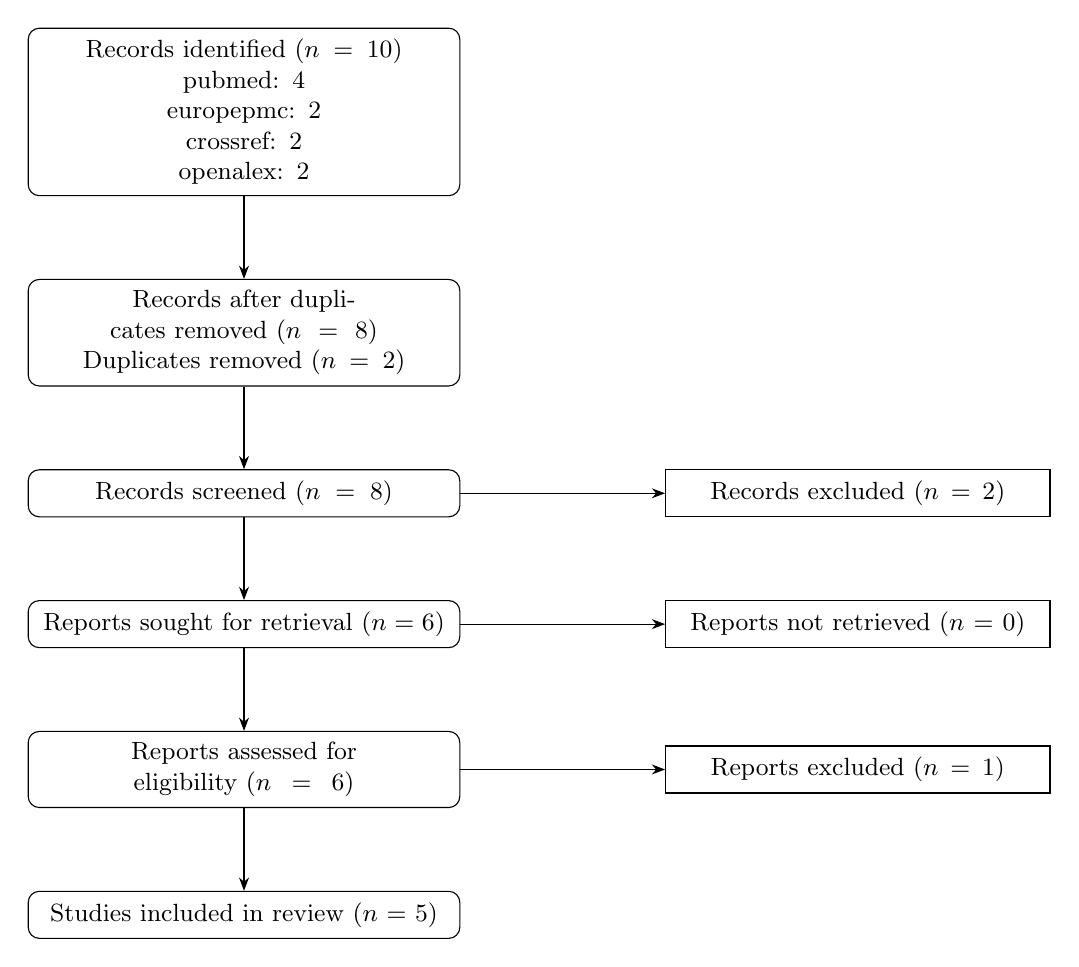
\begin{tikzpicture}[node distance=1.05cm and 2.6cm, box/.style={draw, rounded corners, align=center, text width=5.2cm, inner sep=4pt, font=\small}, side/.style={draw, align=center, text width=4.6cm, inner sep=4pt, font=\small}, >=Stealth]
\node[box] (id) {Records identified ($n=10$)\\ pubmed: 4\\ europepmc: 2\\ crossref: 2\\ openalex: 2};
\node[box, below=of id] (dd) {Records after duplicates removed ($n=8$)\\ Duplicates removed ($n=2$)};
\node[box, below=of dd] (sc) {Records screened ($n=8$)};
\node[side, right=of sc] (ex1) {Records excluded ($n=2$)};
\node[box, below=of sc] (so) {Reports sought for retrieval ($n=6$)};
\node[side, right=of so] (nr) {Reports not retrieved ($n=0$)};
\node[box, below=of so] (as) {Reports assessed for eligibility ($n=6$)};
\node[side, right=of as] (er) {Reports excluded ($n=1$)};
\node[box, below=of as] (in) {Studies included in review ($n=5$)};
\draw[->] (id) -- (dd);
\draw[->] (dd) -- (sc);
\draw[->] (sc) -- (ex1);
\draw[->] (sc) -- (so);
\draw[->] (so) -- (nr);
\draw[->] (so) -- (as);
\draw[->] (as) -- (er);
\draw[->] (as) -- (in);
\end{tikzpicture}
\caption{PRISMA 2020 study-selection flow diagram.}
\end{figure}

5 studies were included \citep{Author2013,Author2015,Author2012,Author2018,Author2016}. The pooled SMD (random effects) was $0.2766$ (95\% CI $0.117$ to $0.4361$; $I^2=0.0\%$, $k=5$). The pooled effect reached significance; heterogeneity was low (I-squared=0.0\%).
\subsection{Characteristics of included studies}
\begin{longtable}{p{3.0cm} l c p{3.2cm} c}
\toprule
Study & Design & $n$ & Population & RoB \\
\midrule
\endhead
Author1 A 2013~\cite{Author2013} & randomized crossover & 52 & Healthy adults & some concerns \\
Author2 A 2015~\cite{Author2015} & randomized crossover & 64 & Healthy adults & some concerns \\
Author3 A 2012~\cite{Author2012} & randomized crossover & 28 & Healthy adults & some concerns \\
Author4 A 2018~\cite{Author2018} & randomized crossover & 40 & Healthy adults & some concerns \\
Author5 A 2016~\cite{Author2016} & randomized crossover & 46 & Healthy adults & some concerns \\
\bottomrule
\caption{Characteristics of included studies.}
\end{longtable}

\subsection{Risk of bias within studies}
\begin{longtable}{p{3.2cm} c c c c c c}
\toprule
Study & \rotatebox{0}{Randomization } & \rotatebox{0}{Deviations} & \rotatebox{0}{Missing outcom} & \rotatebox{0}{Measurement of} & \rotatebox{0}{Selection of t} & Overall \\
\midrule
\endhead
Author1 A 2013 & \cellcolor{roblow}low & \cellcolor{robsome}some concerns & \cellcolor{roblow}low & \cellcolor{robsome}some concerns & \cellcolor{roblow}low & \cellcolor{robsome}some concerns \\
Author2 A 2015 & \cellcolor{roblow}low & \cellcolor{robsome}some concerns & \cellcolor{roblow}low & \cellcolor{robsome}some concerns & \cellcolor{roblow}low & \cellcolor{robsome}some concerns \\
Author3 A 2012 & \cellcolor{roblow}low & \cellcolor{robsome}some concerns & \cellcolor{roblow}low & \cellcolor{robsome}some concerns & \cellcolor{roblow}low & \cellcolor{robsome}some concerns \\
Author4 A 2018 & \cellcolor{roblow}low & \cellcolor{robsome}some concerns & \cellcolor{roblow}low & \cellcolor{robsome}some concerns & \cellcolor{roblow}low & \cellcolor{robsome}some concerns \\
Author5 A 2016 & \cellcolor{roblow}low & \cellcolor{robsome}some concerns & \cellcolor{roblow}low & \cellcolor{robsome}some concerns & \cellcolor{roblow}low & \cellcolor{robsome}some concerns \\
\bottomrule
\caption{Risk-of-bias assessment (RoB2; green = low, amber = some concerns, red = high).}
\end{longtable}

\subsection{Synthesis of results}
\begin{figure}[H]
\centering
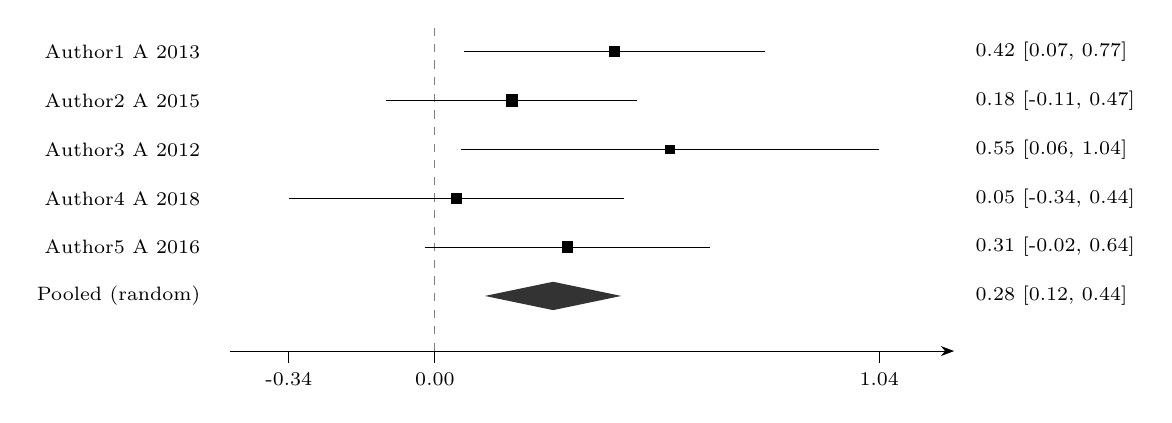
\begin{tikzpicture}[x=1cm,y=1cm,font=\scriptsize,>=Stealth]
\draw[dashed,gray] (2.606,-0.700) -- (2.606,3.400);
\draw[->] (0,-0.700) -- (9.200,-0.700);
\draw (0.750,-0.700) -- (0.750,-0.850) node[below] {-0.34};
\draw (2.606,-0.700) -- (2.606,-0.850) node[below] {0.00};
\draw (8.250,-0.700) -- (8.250,-0.850) node[below] {1.04};
\draw (2.971,3.100) -- (6.800,3.100);
\fill (4.815,3.030) rectangle (4.956,3.171);
\node[left] at (-0.250,3.100) {Author1 A 2013};
\node[right] at (9.350,3.100) {0.42 [0.07, 0.77]};
\draw (1.987,2.480) -- (5.178,2.480);
\fill (3.503,2.401) rectangle (3.662,2.559);
\node[left] at (-0.250,2.480) {Author2 A 2015};
\node[right] at (9.350,2.480) {0.18 [-0.11, 0.47]};
\draw (2.932,1.860) -- (8.250,1.860);
\fill (5.530,1.799) rectangle (5.651,1.921);
\node[left] at (-0.250,1.860) {Author3 A 2012};
\node[right] at (9.350,1.860) {0.55 [0.06, 1.04]};
\draw (0.750,1.240) -- (5.005,1.240);
\fill (2.811,1.173) rectangle (2.944,1.307);
\node[left] at (-0.250,1.240) {Author4 A 2018};
\node[right] at (9.350,1.240) {0.05 [-0.34, 0.44]};
\draw (2.480,0.620) -- (6.097,0.620);
\fill (4.215,0.547) rectangle (4.361,0.693);
\node[left] at (-0.250,0.620) {Author5 A 2016};
\node[right] at (9.350,0.620) {0.31 [-0.02, 0.64]};
\fill[black!80] (3.241,0) -- (4.107,0.18) -- (4.973,0) -- (4.107,-0.18) -- cycle;
\node[left] at (-0.250,0) {Pooled (random)};
\node[right] at (9.350,0) {0.28 [0.12, 0.44]};
\end{tikzpicture}
\caption{Forest plot (SMD, random effects; $k=5$, $I^2=0.0\%$).}
\end{figure}

Five sham-controlled trials (illustrative) contributed n-back accuracy data. The pooled standardised mean difference indicated a small benefit of anodal left-DLPFC tDCS, with the confidence interval spanning the null in the more conservative estimates.
\subsection{Publication bias (PRISMA item 14)}
\begin{figure}[H]
\centering
\begin{tikzpicture}[x=1cm,y=1cm,font=\scriptsize,>=Stealth]
\draw[->] (0,0) -- (8.300,0) node[right] {SMD};
\draw[->] (4.000,0) -- (4.000,5.800) node[above] {precision};
\draw[dashed,gray] (4.000,5.500) -- (0.667,0.000);
\draw[dashed,gray] (4.000,5.500) -- (7.333,0.000);
\draw[dotted] (4.000,0) -- (4.000,5.500);
\fill (4.976,1.540) circle (1.6pt);
\fill (3.343,2.200) circle (1.6pt);
\fill (5.860,0.000) circle (1.6pt);
\fill (2.459,1.100) circle (1.6pt);
\fill (4.227,1.760) circle (1.6pt);
\end{tikzpicture}
\caption{Funnel plot of effect size against precision (apex = pooled estimate; dashed lines = pseudo 95\% confidence funnel).}
\end{figure}

Egger's regression test indicated no strong evidence of funnel asymmetry (intercept $=2.3525$, $p=0.4445$, $k=5$). Note that with $k<10$ the test is under-powered.
\subsection{Certainty of evidence (GRADE)}
\textbf{Certainty: low.} Downgraded for risk of bias (unclear blinding) and imprecision.
\section{Discussion}
The pooled estimate points to a small effect with wide uncertainty. Unclear blinding and small samples temper confidence; results are hypothesis-generating.

\textbf{Limitations.} Small samples, single-session designs, and possible small-study effects.
\section{Conclusions}
Anodal left-DLPFC tDCS may yield a small improvement in n-back accuracy, but certainty is low. Adequately powered, pre-registered trials are needed.
\appendix
\section{PRISMA 2020 checklist}
\begin{longtable}{c p{3.2cm} p{6.0cm} p{3.2cm}}
\toprule
\# & Item & Description & Addressed by \\
\midrule
\endhead
1 & Title & Identify the report as a systematic review. & Title \\
2 & Abstract & See the PRISMA 2020 abstract checklist. & Abstract \\
3 & Rationale & Describe the rationale in the context of existing knowledge. & Background \\
4 & Objectives & Provide an explicit statement of objective(s)/question(s). & ProtocolArchitect \\
5 & Eligibility criteria & Specify inclusion/exclusion criteria and groupings. & ProtocolArchitect \\
6 & Information sources & Specify all databases/registers and the last search date. & SearchStrategist \\
7 & Search strategy & Present full search strategies for all sources. & SearchStrategist / Strategy table \\
8 & Selection process & Methods to decide inclusion (reviewers, independence, tools). & Title/Abstract + Adjudicator \\
9 & Data collection process & Methods to collect data from reports. & DataExtractor \\
10 & Data items & List and define all outcomes and other variables sought. & DataExtractor \\
11 & Study risk of bias assessment & Methods to assess risk of bias. & RiskOfBiasAssessor \\
12 & Effect measures & Specify the effect measure(s) used. & Synthesis config \\
13 & Synthesis methods & Describe processes for synthesis incl. meta-analysis. & EvidenceSynthesizer \\
14 & Reporting bias assessment & Methods to assess risk of bias due to missing results. & EvidenceSynthesizer (publication bias) \\
15 & Certainty assessment & Methods to assess certainty (e.g. GRADE). & RiskOfBiasAssessor (GRADE) \\
16 & Study selection & Report numbers screened/included with a flow diagram. & PRISMA flow diagram \\
17 & Study characteristics & Cite each included study and present its characteristics. & Characteristics table \\
18 & Risk of bias in studies & Present risk-of-bias assessments per study. & Risk-of-bias table \\
19 & Results of individual studies & Present per-study results for each outcome. & Forest / per-study table \\
20 & Results of syntheses & Present results of each synthesis incl. heterogeneity. & Synthesis results \\
21 & Reporting biases & Present assessments of reporting bias. & Discussion (reporting bias) \\
22 & Certainty of evidence & Present certainty (GRADE) for each outcome. & GRADE certainty \\
23 & Discussion & Interpret results; discuss limitations and implications. & Discussion \\
24 & Registration and protocol & Provide registration info / protocol access. & Methods (registration) \\
25 & Support & Describe sources of financial/non-financial support. & Funding \\
26 & Competing interests & Declare competing interests. & Competing interests \\
27 & Availability of data/code & Report availability of data, code, and materials. & Data \& code availability \\
\bottomrule
\caption{PRISMA 2020 checklist.}
\end{longtable}

\bibliographystyle{unsrtnat}
\bibliography{\jobname}
\end{document}
